\section{EXPERIMENTAL SETTING AND RESULTS}
\label{sec:mot}
\begin{figure*}
	\centering
	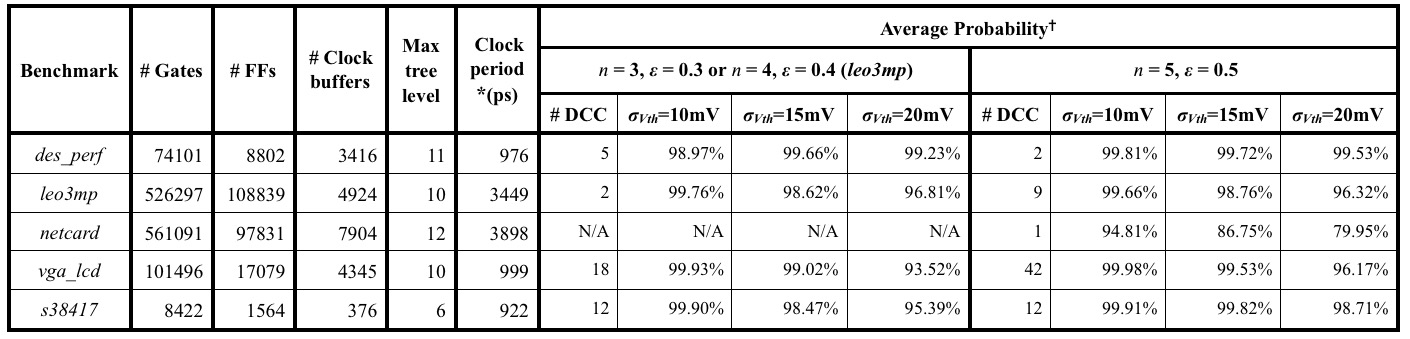
\includegraphics[width=1\columnwidth]{benchmarkinfo.png}
	\caption{Circuit information and estimated lifetime without Trojan insertion}
	\label{fig:benchmark}
\end{figure*}

%%---------TEST--------------
\begin{figure*}[!ht]
    \centering
    \subfigure[\textit{s38417} is attacked with $n$ = 3 yr and $\varepsilon = 0.3$ yr]{
    	\label{fig:sub:s38417_3y}
        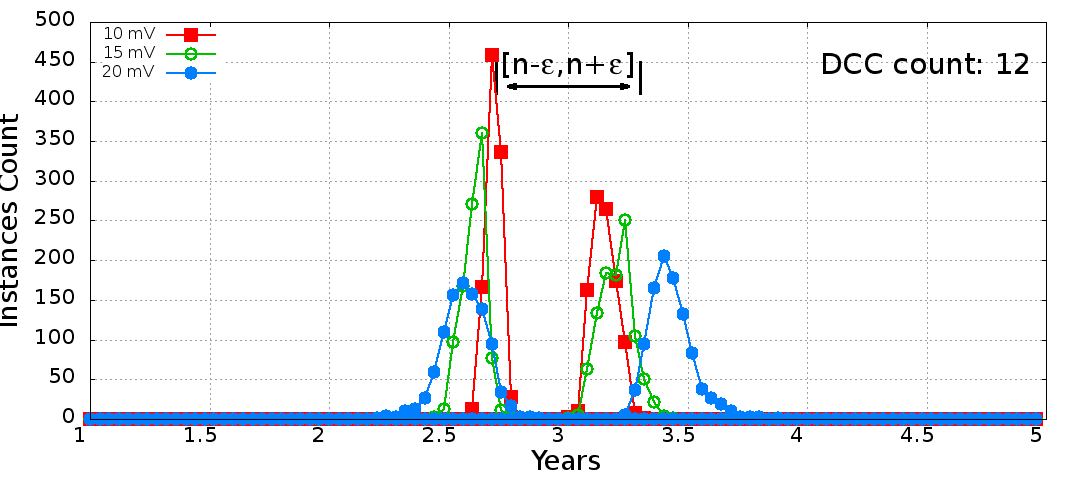
\includegraphics[width=0.7\columnwidth]{s384173y.png}
    }
    \hspace{0.1cm}
    \subfigure[\textit{s38417} is attacked with $n$ = 5 yr and $\varepsilon = 0.5$ yr]{
    	\label{fig:sub:s38417_5y}
        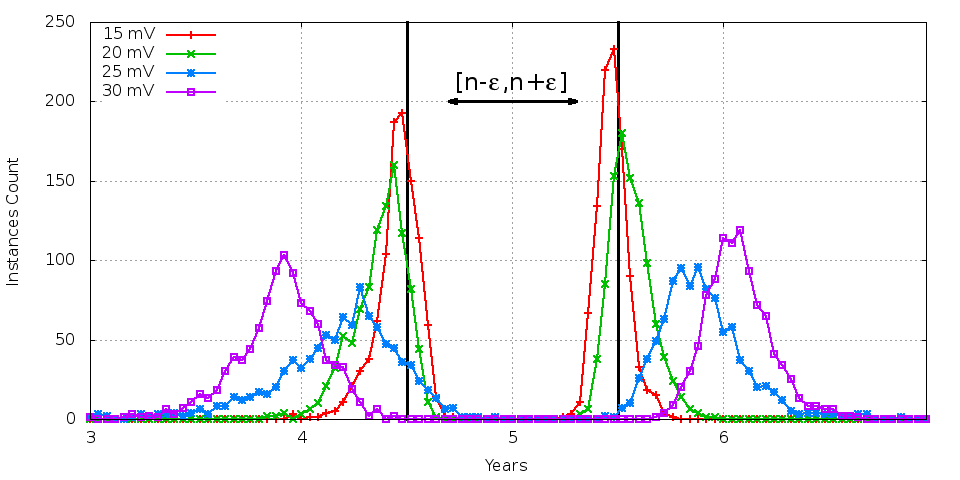
\includegraphics[width=0.7\columnwidth]{s384175y.png}
    }
    \hspace{0.1cm}
    \subfigure[\textit{des\_perf} is attacked with $n$ = 3 yr and $\varepsilon = 0.3$ yr]{
    	\label{fig:sub:des_3y}
        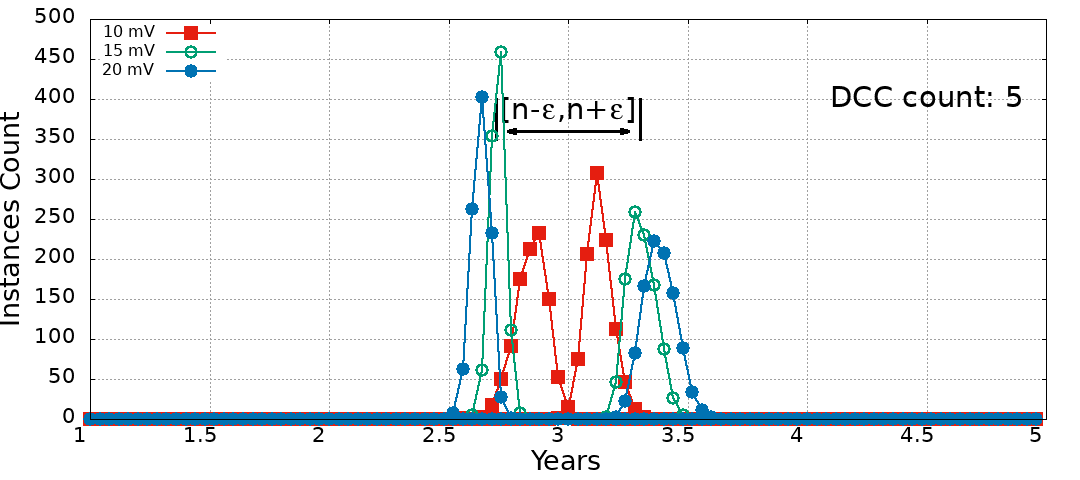
\includegraphics[width=0.7\columnwidth]{des3y.png}
    }
    \subfigure[\textit{des\_perf} is attacked with $n$ = 5 yr and $\varepsilon = 0.5$ yr]{
    	\label{fig:sub:des_5y}
        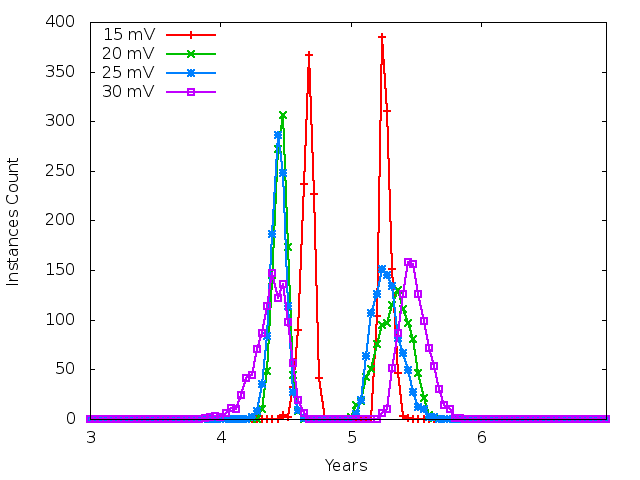
\includegraphics[width=0.7\columnwidth]{des5y.png}
    }
    \subfigure[\textit{leo3mp} is attacked with $n$ = 3 yr and $\varepsilon = 0.3$ yr]{
    	\label{fig:sub:3mp_3y}
        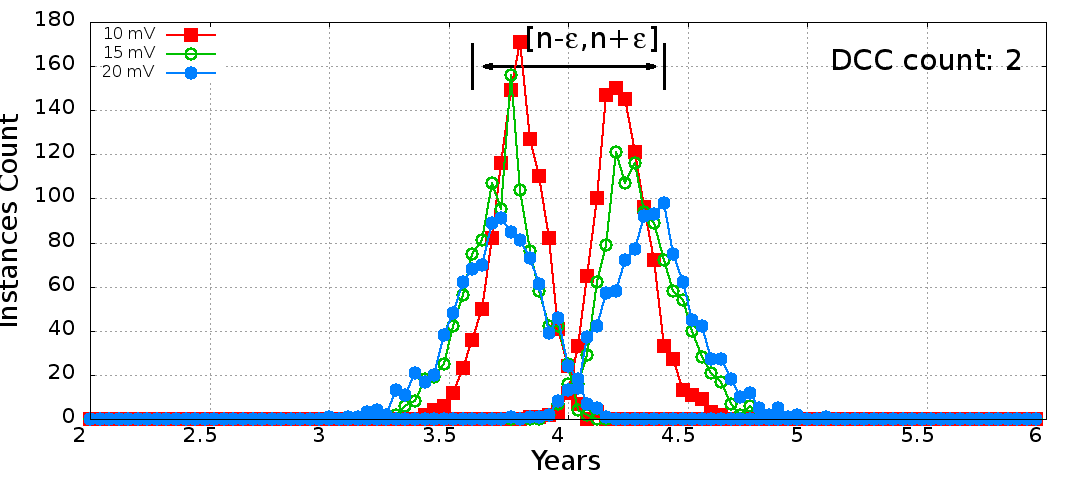
\includegraphics[width=0.7\columnwidth]{3mp4y.png}
    }
    \hspace{0.1cm}
    \subfigure[\textit{leo3mp} is attacked with $n$ = 5 yrs and $\varepsilon = 0.5$ yr]{
    	\label{fig:sub:3mp_5y}
        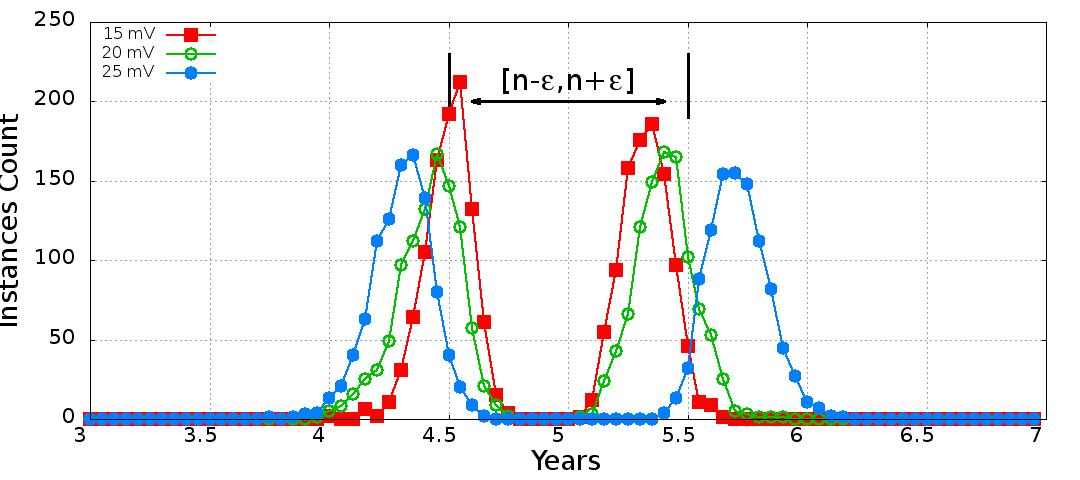
\includegraphics[width=0.7\columnwidth]{3mp5y.png}
    }
    \caption{Lifetime distributions of Monte-Carlo Instances of \textit{s38417}, \textit{des\_perf}, and \textit{leo3mp}}
    \label{fig:exp}
\end{figure*}


In this section, we explain the experimental setting and demonstrate the experimental results of our proposed Trojan attack. The benchmarks in IWLS'05 and ISCAS'89 are used in the experiments. The utilized technology is TSMC 65nm GP standard cell series. The used SAT solver is MiniSAT 2.2. The section is organized as follows: Section~\ref{sec:exp:tc} introduces the experimental setting for clock period. Section~\ref{sec:exp:exp} demonstrates the lifetime distributions of Monte-Carlo instances of attacked designs, Eventually, Section~\ref{sec:exp:det} discuss the detectability of the proposed Trojan attack.  

\subsection{Clock Period Setting}
\label{sec:exp:tc}
Figure \ref{fig:benchmark} shows the lifetime intervals of original (i.e., Trojan-free) designs with clock periods which make the designs fail at a specified time (in our experiment, 7 years) under aging. The resulting clock period is both used in Trojan-free and Trojan-included (attacked) designs. In Figure~\ref{fig:benchmark}, lower bounds are exactly 7 years because circuit clock periods (shown in column 4) are specifically set such that the most critical path, whose slack is smallest, fails at 7th year under the worst-case aging condition. The upper bound of each design differs significantly because, in the Trojan-free designs, only the most critical path is considered for determined the clock period while workload variations are disregarded.

%\subsection{Monte-Carlo Instantiation of the Attacked Designs}
%\label{sec:exp:mc_ins}
%After the locations of DCC insertions are determined, Monte-Carlo simulation is performed to demonstrate the influence of process variation (PV) on the proposed Trojan.

%Given an attacked design, it is instantiated considering PV by imposing extra V\textsubscript{th} offset (i.e., $\Delta V\textsubscript{th}$ ) on each transistor. Note that, these offsets follow a normal distribution with the standard deviation of a given value, which usually ranges from 10mV to 30mV [-19-][-20-]. In other words, if the standard deviation is set to 20mV, it implies that 68\% of V\textsubscript{th} offsets reside between $\pm$ 20mV. Up to present, a Monte-Carlo instance of an attacked design is built.
%Various instances of the attacked design are generated. Each instance (i.e., Monte-Carlo seed) can be considered as a die after the circuit is manufactured. In our experiment, each attacked design is instantiated for 1000 times with a specified standard deviation of V\textsubscript{th}. Whenever an instance is generated, we use aforementioned algorithms to estimate its lifetime interval, which consists of a lower bound and an upper bound.

%\subsection{Lifetime Estimation Considering the Correlation between PVs and Aging}
%\label{sec:exp:cor}
%Whenever an instance is generated, Algorithm~\ref{LT_1} and~\ref{LT_2} are applied to estimate its lifetime. Note that, because PVs is considered, the aging rates of transistors along a path will no longer be equal; in other words, because threshold voltages of transistors along the same path are not fixed, their aging rates differ. Thus, at line 8 in Algorithm~\ref{LT_2}, aging rate of path $i$ ($X_{i}$) must consider the aging rate of individual transistor, instead of using the deterministic Equation (\ref{eq:worst}). It can be modified by following procedures: ($i$) Obtain the aging latency of a path by accumulating gate delays using the above mechanism in part B. ($ii$) Then, aging rate of the path equals the aging latency divided by non-aging/fresh latency.

\subsection{Lifetime Distribution of Monte-Carlo Instances}
\label{sec:exp:exp}
Figure~\ref{fig:exp} shows the lifetime distributions of instances of the attacked three designs (\textit{s38417}, \textit{des\_perf} and \textit{leo3mp}). The designs are attacked to fail at $3^{rd}$, $4^{th}$ or $5^{th}$ year. Note that, there exists no SAT solution while leo3mp is attacked to fail at 3rd year, whereas there exists SAT solution while it is attacked to fail at $4^{th}$ year. In each left/right subfigure, there exist four distributions. The distributions of various colors differ in the standard deviations of V\textsubscript{th} while generating instances. That is, each color corresponds to one distinct value of standard deviation of V\textsubscript{th}. In our experiments, the deviations are set to 15mV, 20mV, 25 mV and 30 mV, respectively. Moreover, in each distribution, there exist two peaks. The left/right peak denotes the distribution of lower/upper bounds of lifetime intervals of instances. Note that, there exist two differences between Figure~\ref{fig:benchmark} and the Figure~\ref{fig:exp}. First, the designs in Figure~\ref{fig:benchmark} are Trojan-free ones, instead of Trojan-included ones in Figure~\ref{fig:exp}. Second, because the lifetime intervals of the Trojan-free designs are not subject to the process variations, the original lifetime intervals ($5^{th}$ column in Figure~\ref{fig:benchmark}) do not consider the effect of PVs.
Apparently, Figure~\ref{fig:exp} shows that, as the standard deviation becomes larger, the interval between the left and right peaks becomes wider; that is, the larger standard deviation leads to a less accurate attack. Therefore, the lifetime accuracy of the proposed Trojan is impacted by the diversity of threshold voltages. However, even though the peaks of two bounds deviate from the desired lifetime interval $[n - \varepsilon, n + \varepsilon]$, it does not mean that the attacked designs must not fail in that interval. As mentioned in Section~\ref{sec:lt_estimation}, the estimated lifetime interval of one instance consists of two bounds. One is lower bound; and the other is upper bound. The two bounds denote the earliest and the last time points, at which the instance will fail. But the exact time point, at which the instance fails, depends on the workload. Therefore, since the lifetime interval of each instance is overlapped with the desired lifetime interval $[n - \varepsilon, n + \varepsilon]$, the proposed Trojan is still likely to control the design lifetime in that interval.

\subsection{Detectability}
\label{sec:exp:det}
When it comes to the detectability of the proposed Trojan, side-channel analysis is often used to detect the existence of hardware Trojan. Nevertheless, the used DCC count is marginal compared with the total gate count. On average, DCC count is less than 0.2\% of total gate count. That is, the area overhead is insignificant. Also, the power overhead due to DCCs can be regarded as the power variations caused by PV. Therefore, the proposed Trojan framework is difficult to be detected by conventional side-channel analysis.
Some Trojan defenders can insert probes in the clock network to inspect the variation of clock duty cycle. The detection method is indeed able to prove the existence of the proposed Trojan. However, the method need to be supported by extra I/O pins/ports. Therefore, it is impractical, not only because the pin counts of ICs are limited, but also the area over- head of extra pins is costly.

\section{CONCLUSION}
We proposed a methodology of hardware Trojan insertion to control the circuit lifetime with the consideration of aging behavior, correlation between pairs of critical paths and process variations. The influence of Trojan heavily reduce the lifetime of circuit instances. Even though the accuracy is impacted by PVs, the lifetime of instances is still likely to fail within the desired lifetime interval $[n - \varepsilon, n + \varepsilon]$. Also, the DCC count is less than 0.2\% of total gate count, implying limited area and power overhead. Therefore, the proposed Trojan is difficult to be detected.
